\documentclass{standalone}

\usepackage{tikz,tikz-3dplot,pgfplots,xcolor}
\usetikzlibrary{arrows.meta,calc}

%\pgfplotsset{compat=1.18} 
\definecolor{gray0}{rgb}{0.98,0.98,0.98}
\definecolor{gray1}{rgb}{0.8,0.8,0.8}
\definecolor{gray2}{rgb}{0.7,0.7,0.7}

\begin{document}

  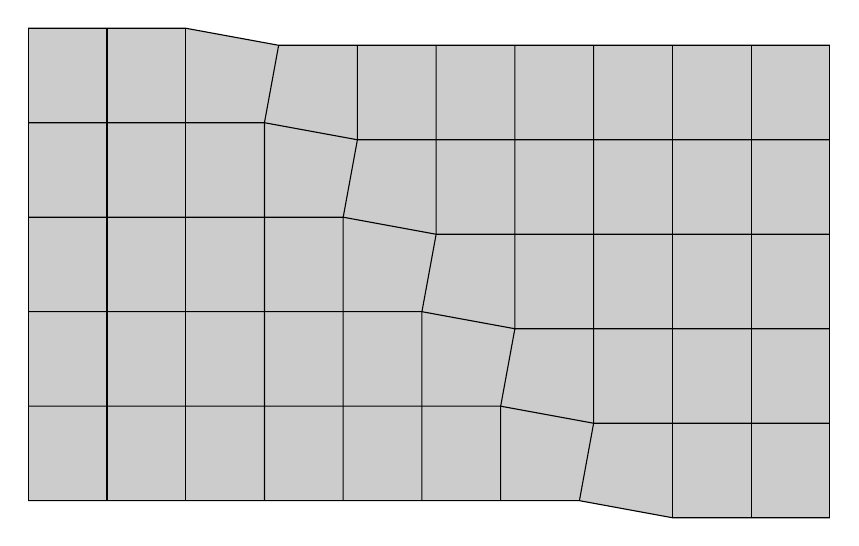
\begin{tikzpicture}[>=Latex]

    \path[fill=gray1] (0,0) --++ (7,0) --++ (-10.4:1.2)--++(2,0)--++(0,6)--++(-7,0)--++(169.6:1.2)--++(-2,0)--cycle;
    \draw (0,0) --++ (0,6);
    \draw (1,0) --++ (0,6);
    \draw (2,0) --++ (0,6);
    \draw (3,0) --++ (0,4.8) --++ (79.6:1);
    \draw (4,0) --++ (0,3.6) --++ (79.6:1) --++ (0,1.2);
    \draw (5,0) --++ (0,2.4) --++ (79.6:1) --++ (0,2.4);
    \draw (6,0) --++ (0,1.2) --++ (79.6:1) --++ (0,3.6);
    \draw (7,0) --++ (79.6:1) --++ (0,4.8);
    \path (7,0) --++ (-10.4:1.2) coordinate(co1)--++(1,0)coordinate(co2)--++(1,0)coordinate(co3);
    \draw (co1) --++ (0,6);
    \draw (co2) --++ (0,6);
    \draw (co3) --++ (0,6);
    \draw (0,0)  --++(7,0)--++(-10.4:1.2)--++(2,0);
    \draw (0,1.2)--++(6,0)--++(-10.4:1.2)--++(3,0);
    \draw (0,2.4)--++(5,0)--++(-10.4:1.2)--++(4,0);
    \draw (0,3.6)--++(4,0)--++(-10.4:1.2)--++(5,0);
    \draw (0,4.8)--++(3,0)--++(-10.4:1.2)--++(6,0);
    \draw (0,6)  --++(2,0)--++(-10.4:1.2)--++(7,0);

  \end{tikzpicture}
\end{document}